
\documentclass[journal]{IEEEtran}
\usepackage{blindtext}
\usepackage{graphicx}
\usepackage{xcolor}% you could also use the color package
\usepackage{colortbl}
\usepackage{varioref}
\usepackage{placeins}
\usepackage{listings}
\usepackage{color}

\definecolor{dkgreen}{rgb}{0,0.6,0}
\definecolor{gray}{rgb}{0.5,0.5,0.5}
\definecolor{mauve}{rgb}{0.58,0,0.82}

\lstset{frame=tb,
  language=C,
  aboveskip=3mm,
  belowskip=3mm,
  showstringspaces=false,
  columns=flexible,
  basicstyle={\small\ttfamily},
  numbers=none,
  numberstyle=\tiny\color{gray},
  keywordstyle=\color{blue},
  commentstyle=\color{dkgreen},
  stringstyle=\color{mauve},
  breaklines=true,
  breakatwhitespace=true,
  tabsize=3
}







% *** GRAPHICS RELATED PACKAGES ***
%
\ifCLASSINFOpdf

\else

\fi


% correct bad hyphenation here
\hyphenation{op-tical net-works semi-conduc-tor}


\begin{document}
%
% paper title
% can use linebreaks \\ within to get better formatting as desired
\title{Advanced Architectures Assignment}

\author{Alexandre~Silva
        and~Daniel~Malhadas}% <-this % stops a space

% The paper headers
\markboth{University of Minho, Parallel and Distributed Computing, 2016/2017}%
{Shell \MakeLowercase{\textit{et al.}}: University of Minho, 2016/2017}


% make the title area
\maketitle


\begin{abstract}
This journal reports the effort and work expended by the authors in order to reach conclusions regarding the efficiency and quality between different implementations of multiplications of square matrices. The classical implementation of matrix multiplication consists of three loops and the index of each one will refer to different components, being the lines(i), columns(j) and accumulation of multiplications for each value of the resulting matrix(k). The different implementations referred to above consist of changing the order of these indexes. On this project three different variations for this order were studied, these being ijk, ikj and jki. Further instrumentation provided the needed results to compare these three in terms of efficiency and result quality in different computational environments (single-threaded, multi-threaded, Xeon processor, Xeon Phi co-processor). In order to be able to proceed with said instrumentation we used a library written in C that goes by the name of PAPI.
%\boldmath
%\blindtext[1]
\end{abstract}

\begin{IEEEkeywords}
PAPI, Square Matrices Multiplication, Parallel and Distributed Computing, Roofline Model, Xeon, Xeon Phi.
\end{IEEEkeywords}




\IEEEpeerreviewmaketitle

\section{Initial considerations}
\subsection{Machine characterization}
During this assignment two main machines were used and the 
results presented from now on will be related to these 
specific machines. The use of two different machines allows 
for a much better understanding and certainty from the 
results of our studies since we get results from two 
fundamentally different kinds of machine. Our machines are: 
a personal laptop and Cluster SeARCH's node 652. Both these 
machines are fully characterized on the next table:\\
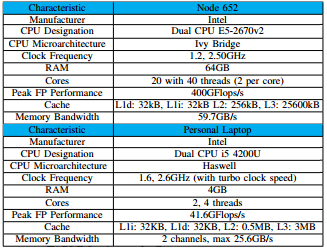
\includegraphics[width=0.5\textwidth]{comps.png}

This data was obtained from various places. By using the Unix command \textbf{lscpu}, it allowed us to know the manufacturer, number of cores and threads per core and size of cache levels. For the remaining items we visited cpu-world.com and ark.intel.com.

\subsection{PAPI Instrumentation}
Performance Application Programming Interface (PAPI) is a tool that we used to instrument our code. It allows us to access relevant CPU performance counters that we will use to measure our code's performance and quality. By using the command \textbf{papi\_avail} on PAPI version 5.5.0.0 we got information about all counters. From those the ones we choose as relevant to analyse an application execution time and to identify potential bottlenecks are presented on the next table:

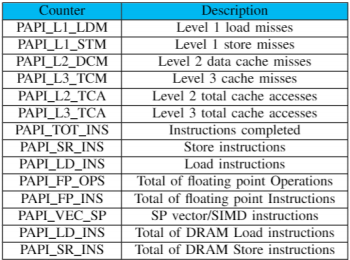
\includegraphics[width=0.35\textwidth]{paps.png}

It's important to note that some of these counters are not compatible with each other when measured together, therefore we used the command \textbf{papi\_event\_chooser} followed by the counters we wanted to use which tells us if any of them is incompatible with the others. Using this we were able to make various measurements of our code using different compatible counters each time and were able to get the different values that way. Even though now we can measure all counters we wanted we loose some fidelity and quality on the results given by them because we will compare them with others that were measured at different times in different measurements of our code however this was the best solutions we could find and therefore interpret it as a necessary induced break in the overall fidelity of the results presented on the next sections of this document.\\
These counters were the ones that looked the most relevant because with just these we can measure various different possible bottlenecks. From these counters we can derive: \textbf{ Percentage of miss rate on any cache level}, Bottlenecks that result from the lack of good programming taking into account the hardware and how it works can be calculated through miss rates on the various cache levels. We interpret miss rate percentage on a certain level as: from all cache accesses on that level, the percentage that was a miss. Taking as an example a matrix being accessed column by column like we saw on section 1, we can guess that we will have a higher miss rate on cache L1 than if the matrix was accessed by rows. Therefore miss rates can be valuable when trying to understand if our code is indeed making good use of the cache or if we have to change something in order to have less misses that may impact performance. We can derive the following formula with the previous counters: \textbf{MissRatePercentage = PAPI\_LX\_TCM/PAPI\_LX\_TCA *100}, being X the cache level. However the miss rate on cache L1 cannot be calculated because, even though PAPI\_L1\_TCA is available on the 652 node (verifiable by using the command \textbf{papi\_avail}) when we use the command \textbf{papi\_event\_chooser NATIVE PAPI\_L1\_TCA} we get the following message: "Event PAPI\_L1\_TCA can't be counted with others -7" however this event is the only one used as an argument so we do not understand what we may be doing wrong. Because we were unable to solve this issue we were unable to calculate cache L1's miss rate percentage from the first formula so a different one was used \textbf{(PAPI\_L1\_LDM+PAPI\_L1\_STM)/(PAPI\_SR\_INS}\\
\textbf{+PAPI\_LD\_INS)}, this formula works because we know that every load or store can only be done after an access to cache level 1 regardless of the level it's actually stored from or loaded to, therefore PAPI\_SR\_INS+PAPI\_LD\_INS is a good approximation of total cache L1 accesses.\\ From these counters we can also measure \textbf{Number of RAM accesses per instruction}, can be calculated with the following formula: \textbf{RamAccessesPerInstruction = PAPI\_LD\_INS/PAPI\_FP\_INS}, this number allows us to understand how frequent memory accesses are in comparison to instructions relevant to our code (in this code, instructions regarding floats, because our matrices are composed by floats). It is known that memory accesses can easily become a huge bottleneck if the programmer is not careful therefore it's important to measure it. \textbf{BytesTo/FromRam},can be calculated with the following formula: \textbf{BytesTo/FromRam = CacheLineSize*PAPI\_LD\_INS + CacheLineSize*PAPI\_SR\_INS}. and also \textbf{- Operational Intensity} = \textbf{PAPI\_FP\_OPS/(CacheLineSize*PAPI\_L3\_TCM)} and \textbf{- GFlops/second} \textbf{= ((PAPI\_FP\_OPS+(PAPI\_VEC\_SP*(SIMD\_width /CacheLineSize)))/(Executiontime(microseconds)∗10\^−6))/10\^9}, witch will be usefull fo the roofline graph (explained on the next sub-section.

\subsection{Roofline Model}
As mentioned before we will compare results between two very different machines. In order to be able to compare them and understand which is faster we will use a performance evaluation model called \textbf{Roofline Model}. This model allows us to estimate peak performance. With this we can understand the performance limitations of the current machine and, by plotting the achieved performance on said graph we can determine if our code is CPU-Bound or Memory-Bound. Peak performance was calculated like this: maxClockFrequency*FMA*SIMD*#cores*#CPU. Maximum memory bandwith can then be calculated like this: PeakPerformance/respectiveOperationalIntensity, this formula allows us to know what's the OperationalIntensity on peakPerformance. The next graph shows peak performance for this situation with our two machines:
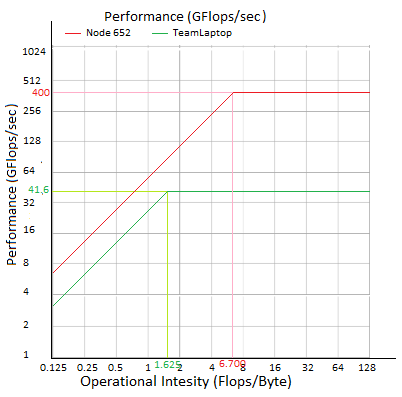
\includegraphics[width=0.5\textwidth]{roof1.png}
 After gathering this information we were able to define ceilings for the roofline model our team's laptop. The team decided that the following CPU ceilings were relevant (ordered by the easiest to obtain to the hardest): an FMA/MAC ceiling GFlop/sec limit without FMA or MAC, ILP ceiling demonstrating GFlops/sec without ILP and a SIMD ceiling demonstrating the GFlop/sec limit without SIMD. We also added memory ceilings (ordered from easiest to obtain to hardest): A ceiling demonstrating performance limitations without SW prefetch and a ceiling demonstrating performance limitations without NUMA architecture.
 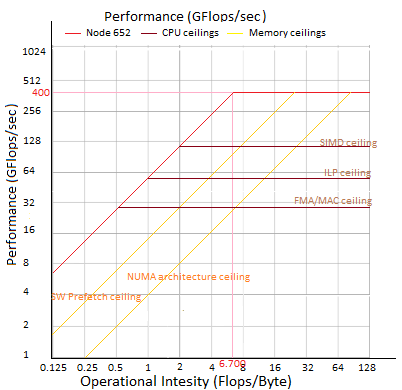
\includegraphics[width=0.35\textwidth]{roof4.png}






\section{Initial Implementations}
During the assignment we were asked to implement three different matrices multiplication algorithms for  square matrices in the canonical form \textbf{A*B=C}, in single precision. The first approach consists of a single-threaded environment and no block optimization. The classical implementation of matrix multiplication consists of three loops and the index of each one will refer to different components, being the lines(i), columns(j) and accumulation of multiplications for each value of the resulting matrix(k). The different implementations referred to above consist of changing the order of these indexes. On this project three different variations for this order were studied, these being ijk, ikj and jki. All of the versions receive three pointers, each referring to one of the different matrices and the size of each (as they are square, just one size is needed for both rows and collumns). It is also to be noted that matrix A is initialized with random single precision values, B with all elements as ones and C all zeros.\\
The first implementation we did was with index order ijk and it's implementation's code is now presented and explained:
\begin{lstlisting}
void matMult_ijk(float **A,float **B,float **C,float N){
    float i,j,k;
    for ( i = 0 ; i < N ; i++ ) {
        for ( j = 0 ; j < N ; j++ ) {
            for ( k = 0 ; k < N ; k++ )
                C[i][j] += A[i][k]*B[k][j];
        }
    }
}
\end{lstlisting}

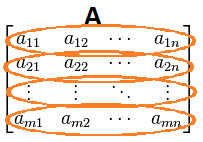
\includegraphics[width=0.15\textwidth, left]{A_row.png}
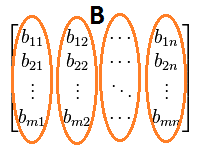
\includegraphics[width=0.15\textwidth, right]{B_column.png}

There is nothing much we can do here to optimize without dividing the matrix in blocks, vectorization, multi-threading, etc. this is as simple as it gets, just the three classic loops as described above. On this algorithm we have four matrix accesses per inner loop iteration and we can notice that while matrix A and C values are accessed by rows, matrix B is accessed by columns. This means look ups for values of matrix B are more expensive in terms of memory then look ups on matrix A as they are not accessed in contiguous memory. 
Now we look into the implementation with ikj index order:
\begin{lstlisting}
void matMult_ikj(float **A,float **B,float **C,float N){
    float i,j,k,*iRowA,*iRowC,*kRowB,ikA;
    for ( i = 0 ; i < N ; i++ ) {
        iRowA = A[i];
        iRowC = C[i];
        for ( k = 0 ; k < N ; k++ ) {
            kRowB = B[k];
            ikA   = iRowA[k];
            for ( j = 0 ; j < N ; j++ )
                iRowC[j] += ikA * kRowB[j];
        }
    }
}
\end{lstlisting}

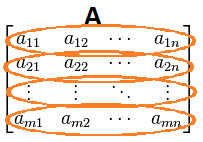
\includegraphics[width=0.15\textwidth, left]{A_row.png}
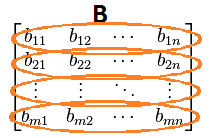
\includegraphics[width=0.15\textwidth, right]{B_row.png}

This time we access matrices elements row by row in contiguous memory therefore we don't have the performance problem with memory accesses like in the previous version. We can also exploit the fact that the second loop is running with it's index as k to do some calculations that would otherwise have to be done for each iteration of the third loop. This way we minimize possible overhead of having to look up for matrices values that would be exactly the same as in the previous iteration. The matrix that benefits the most from this optimization is matrix A, as we see it is never accessed on the third loop, the relevant value was already stored on a local temporary variable.\\
Finally we look into jki index order:
\begin{lstlisting}
void matMult_jki(float **A,float **B,float **C,float N){
    float i,j,k,temp;
    for ( j = 0 ; j < N ; j++ ) {
        for ( k = 0 ; k < N ; k++ ) {
            temp = B[k][j];
            for ( i = 0 ; i < N ; i++ )
                C[i][j] += A[i][k]*temp;
        }
    }
}
\end{lstlisting}

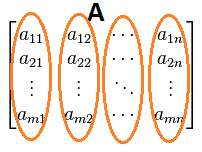
\includegraphics[width=0.15\textwidth, left]{A_column.png}
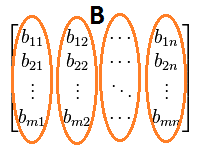
\includegraphics[width=0.15\textwidth, right]{B_column.png}

While this version allows to save on a local variable a value from the matrix B reducing the look ups of values from that matrix in the third loop, like we did for matrix A in the previous version, we can also note that all three matrices are now accessed by columns instead of rows which means it's elements are not being accessed in contiguous memory.  This will make look ups of values of matrices more "expensive" in terms of memory access therefore reducing the performance. In order to solve this, a possible solution is to transpose the problematic matrices, in this case we should transpose A and B. This way, the elements that were previously on different rows but same columns will now be on the same row and different columns allowing us to access them contiguously. We now present a modified version of this multiplication where we receive the already transposed matrices A and B and reflect upon this transposed nature on the way we access it's values in order to achieve the same result as we would do with the other versions.
\begin{lstlisting}
void matMultTranspose_jki(float **A,float **B,float **C,float N){
    float i,j,k,temp;
    for ( j = 0 ; j < N ; j++ ) {
        for ( k = 0 ; k < N ; k++ ) {
            temp = B[j][k];
            for ( i = 0 ; i < N ; i++ )
                C[i][j] += A[k][i]*temp;
        }
    }
}
\end{lstlisting}

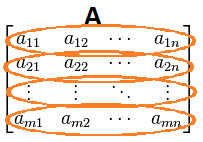
\includegraphics[width=0.15\textwidth, left]{A_row.png}
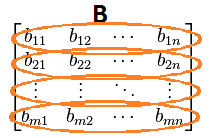
\includegraphics[width=0.15\textwidth, right]{B_row.png}

This way, by switching the indexes we use to access line and column of matrix A([i][k] to [k][i]) and B([k][j] to [j][k]) and taking into account A and B here are the transpose of A and B, we no longer are accessing A's or B's values by columns and solved our performance problem with this version.\\

Now that we deepened our understanding on the good and the not so good about these implementations it's important to also gather relevant information in order to understand appropriate sizes for matrices A, B and C (obviously all three will have the same size) so that our performance tests are indeed relevant and not just random cases chosen arbitrarily. four relevant data-sets were chosen:\\
\textbf{1 - One data-set that completely fits in L1 Cache}\\
The 652 Cluster's node described on the previous section has L1d: 32kB and L1i: 32kB, we only care about data therefore we have a total of 32kB on cache L1 for our data. Each single precision value on each matrix (float) will need 4 bytes, therefore on this cache level we can store 32000B/4B=8000 floats. We have 3 matrices, if we want them all to fit on cache L1 then each must have a maximum of 8000/3=2666.(6) elements, so sqrt(2666.(6))=51.64 is the maximum number of floats per dimension, however we can't have 0.03 float so we have to round it down to 51 per dimension. But it's not over yet as we can also take into account the size of a cache line. In this case it is 64B, therefore we can fit 16 floats on a cache line, so our total number of floats per matrix must be a multiple of 16 in order to improve spacial locality on the cache. 51*51/16=162.56 therefore it's not multiple, we then have to find the closest number to 51 (and smaller of course) that meets this condition, that number is 48 (48*48/16=144). In short: max dimensions per matrix are 51*51\\
\underline{ideal dimensions are 48*48}\\ 
the next data-sets were calculated in a similar manner.\\
\textbf{2 - One data-set that completely fits in L2 Cache}\\
max dimensions per matrix are 146*146\\
\underline{ideal dimensions are 144*144}\\ 
\textbf{3 - One data-set that completely fits in L3 Cache}\\
max dimensions per matrix are 1460*1460,\\
\underline{ideal dimensions are 1456*1456}\\ 
\textbf{4 - One data-set that cannot fit on the previous cache levels and forces CPU to load it from DRAM}\\
Here we just need a bigger size then 1460*1460, but we will try to find a significant one that has a number of floats per matrix multiple of the 16 floats we can fit in each cache line.
\underline{good relevant dimensions are 2000*2000}


\section{Measuring Performance of Initial Implementations}

Now that the data-sets are established they are used to compare execution times between the different implementations with various input sizes. In order to measure execution time the function \textbf{PAPI\_get\_real\_usec()} was used. this function returns a long long int that represents time in micro seconds. Because it is a long long int we can trust in all digits that are shown as none of them crosses the maximum number of viable digits. Also in an attempt to reduce abrupt spikes on the graph shown below we use a logarithmic scale on Y axis. It is to be noted that the version that uses transposed matrices also takes into account the time of transposing, otherwise it would not be a fair comparison with the other versions because this transposing is also an important step to correctly proceed with the multiplication.\\
The next graph shows for all implementations explained on the previous section an average of the execution time for a certain data-set:
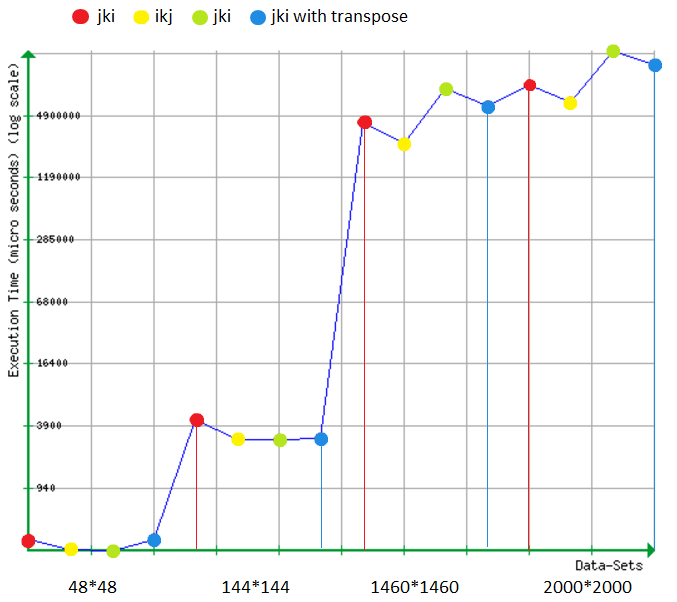
\includegraphics[width=0.50\textwidth,left]{tt.png}
A table with execution times for all implementations for each data-set following the K-best scheme, with K=3 with 5\% tolerance and at most 8 execution times is now shown:\\
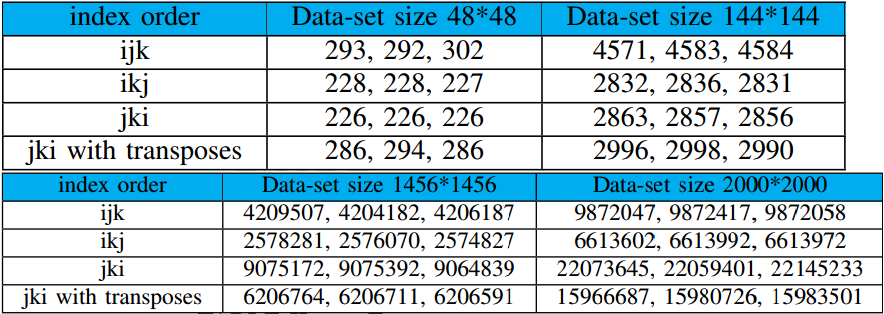
\includegraphics[width=0.50\textwidth, left]{tempinhos.png}

With these values we prove that the index order jki with transpose of matrices is indeed faster then just jki without transposes even though this doesn't happen for the two smallest data-sets (probably because they are too small to ever justify the need for local spatiality and for that reason the overhead caused by calculating the transposes overshadows any possible gain). We also notice that ikj is the fastest in average with ijk standing in middle ground. All this we estimated on section 2 when we pondered about the way each implementation accessed the matrices.\\ 
\\
Now for the best execution time found of each implementation with each data-set we will measure what was the RAM accesses per instruction and the number of bytes transferred to/from the RAM. This can easily be done with the formulas that use PAPI counters presented on section 1 however we will first try to estimate what the results will be. For the first data size we will have a total of 48*48 numbers per matrix witch means we will do 48*48*48=110592 iterations of the inner loop. We know that per each iteration, our matrices are accessed four times, one for A and B and two for C. One of this accesses will be a store (store value in C) and the other three will be loads (load value from C, B and A). This means in total there will be 110592 stores and 110592*3=331776 loads. We also know cache will be warm because multiplications are done right after generating random values for matrix A, filling B with ones and C with zeros. Because of this A and B accesses are assumed not to reach RAM as they should already be in cache and shouldn't "disappear" because they are never changed, just accessed. However matrix C is indeed changed and therefore has to be stored in RAM every time it happens to maintain cache coherence. As it was just changed we believe that it will be already stored on cache so when we access C next time we won't need to load it from RAM. We also know that because our cache has 64B per line, that will be the amount transferred to/from each time RAM is accessed. In conclusion 64*8*110592=56623104bytes is the estimated value transferred to/from RAM. With this we also notice that for each iteration of the inner loop we will have one load from RAM and two floating point operations (one multiplication between value of A and B, sum of that multiplication with previous value of C) therefore we will have a ratio of 0.5 Ram accesses per instruction.\\
For the second and third data-sets (the ones that fit into cache L2 and L3 respectively) we believe this ratio won't change. We also believe bytes transferred to/from RAM can be  calculated the same way, we just need to change the number of iterations. with this logic, for the second data-set we believe will be transferred to/from RAM 64*8*144*144*144=1528823808bytes and for the third it will be 64*8*1460*1460*1460=1593413632000bytes. For the last data-set we will have a total of 2000*2000*3*4*8=384000000bytes however cache L3 only has 25600*1024*8=209715200bytes witch means at least 384000000-209715200=174284800bytes will have to be transferred from RAM eventually. We also still have to store C on RAM in each iteration. Finally we have 174284800+64*8*2000*2000*2000=4096174284800bytes transferred to/from memory.\\
Now we finally calculate the real values using PAPI counters as states on section 1 and compare them with our expected results:\\

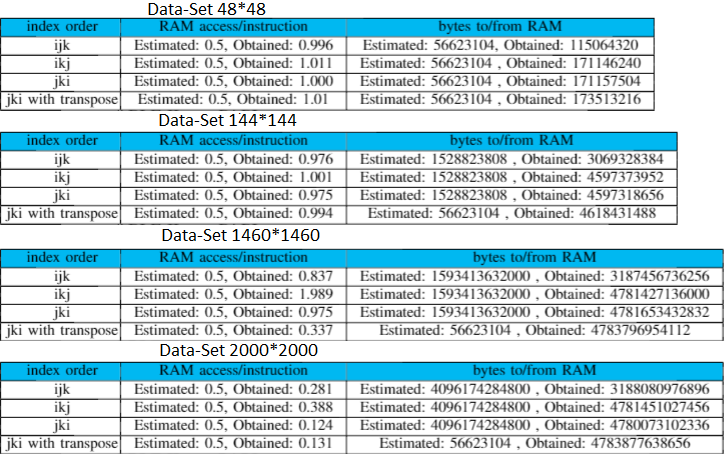
\includegraphics[width=0.50\textwidth, left]{tebelinhas.png}

By looking at these tables it is noticeable that our estimations were missing something. They are correct but not complete. As we see instead of having one RAM access per instruction we actually have, in the majority of cases, one RAM access per one instruction. This means that there may be one more RAM access besides the store of matrix C that we predicted. If there truly is one more then the values for bytes transferred to/from RAM actually back it up because they seem to be, in average, a rough approximation of two times what we predicted it would be.\\
\\
Now we estimate how many FP operations we will have with each data-set for each implementation. We already stated above that per inner loop iteration there will be two FP operations (one multiplication between value of A and B and sum of that multiplication with previous value of C). Therefore we can calculate the total FP operations like this: FP operations per iteration * number of iterations. We know present our estimations and validate them by using PAPI counters while also presenting values for GFlops/sec in order to plot our achieved performance in the roofline graph:

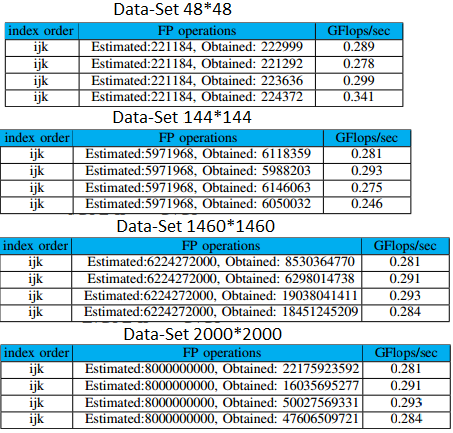
\includegraphics[width=0.50\textwidth, left]{flop.png}

Cache miss rates were also measured and presented on the next table:

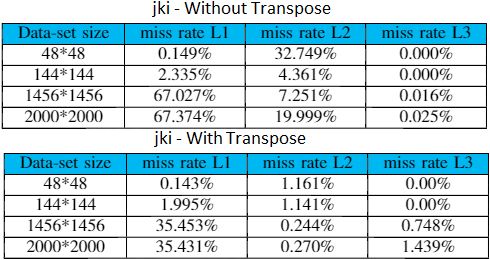
\includegraphics[width=0.50\textwidth, left]{cache.png}

As was expected, for the first data-set there are almost no misses on L1, the same for the second Data-Set with L2. We also notice the first three data-sets have a miss rate on L3 very close to zero, this was expected because all these three sets fit within L1, L2 and L3. However one of the values was different then expected, cache miss rate on L3 for the biggest data-set seems too low, this data-set is bigger then L3 so the miss rate should be considerable and not close to zero. We believe this may have happened because the data-set was perhaps too small to actually show the effects of being bigger then L3. With a bigger data-set, perhaps 4000*4000 this should be more noticeable. It is to also be noted that the version with transpose tends to have a smaller miss rate in all cache levels then the version without transpose. This was also expected because on the version with transpose we are accessing contiguous memory addresses and therefore are able to take advantage of local local spatiality.

\section{Further Optimizations}
\\
\textbf{NOTE}:code demonstrating the optimizations that will be shown below is presented on appendix A.
\\
\subsection{Block Optimization}
For data-sets much bigger then any cache level we may have trouble trying to make good use of the cache with these implementations. We may have matrices so big that one line may be bigger then all cache levels so in consequent iterations we will have to reload matrices elements that we had previously on cache (however had to replace them with others in the last multiplication). This constant reloading sounds like a waste and actually can be reduced by using block optimization. With this we divide the matrix in various blocks of equal size that fit our cache and for each block we do all calculations that we need with those values in order not to have to reload them again. After this, the result of the operations on all blocks is combined and the final matrix is formed. The value for the block size is important as it will define how good our optimization actually is. It has to be smaller then cache levels and the matrix size has to be perfectly divided by this block size (so that all blocks have the same size). We also believe it is good ifit is a multiple of the floats that fit into a cache line. Because we can fit 16 floats in this specific case we chose 8 as our block size as it was the size that brought us the best performance. 

\subsection{Vectorization}

This code contains the right ingredients for vectorization. We tried to vectorize it compiling with the following command \textbf{gcc -O2 -ftree-vectorize -fopt-info-vec-all.} however it couldn't vectorize so we had to force it. For this we used various techniques like aligned our matrices with \textbf{\_\_attribute\_\_ ((aligned))} 

\subsection{Paralelization}

With the intention of running this code efficiently in all cores of the multicore devices of one 652 node we used OMP. We identified each block operations independent to the other blocks, therefore we can divide our threads and have each one deal with a different set of blocks. Because our matrices have a dimension multiple of the blocksize we should also have a number of threads multiple with that number, this way we can allow all threads to operate over the same number of blocks so that the data is well balanced between them. Because we only have 20 threads without HyperThreading we decided to use 16 threads. Also, to guarantee all threads operate over the same number of blocks we use a parallel for with schedule(static,setOfBlocks), with \textbf{setOfBlocks = (n/BlockSize)/Nthreads}. The code is shown below:

\subsection{Offload to Xeon Phi manycore co-processor}

On this section we offload to the manycore co-processor on node 652. By doing this we are able to use all of it's cores to have a bigger number of threads to paralyze the outer loop. We also adapt the number of threads taking into consideration that now we have access to more cores and can afford to have more threads.
\section{Conclusions}
In conclusion we see the initial implementations plotted on the roofline model on appendix B as well as comparison between the optimizations execution time and the initial versions on the following table:
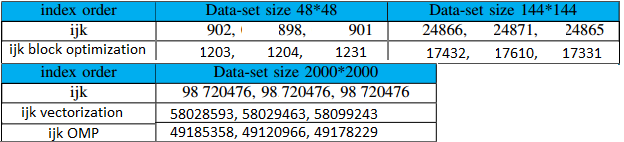
\includegraphics[width=0.50\textwidth, left]{vala.png}
we expected all implementations to be CPU bound except from the ones that utilize the last data-set because it is bigger then all cache levels and it is expected to have much more RAM accesses, however this is not what we observe with the roofline graph. We think this happens simply because our data-set 2000*2000 was to small for the bottleneck from RAM accesses to be noticeable.\\
After looking at the execution times on the table we also see that we actually get better results with the optimized versions. We get better performance from the OMP version then the vectorized version like was expected and believe it to be proof of a good division of the data space between threads. we also believe the better time execution on the vectorized version and the block version in relation to the initial one came from a good choice of block size.


\appendix %

\section*{Appendix A}
\\
\textbf{Block Optimization Code}
\\
\begin{lstlisting}
void matMultBlock(float **a,float **b,float **c,float n) {
	int i1, j1, k1, i, j, k;
	for( i1=0;i1<n; i1= i1 + BlockSize) {
		for(j1=0;j1<n; j1 = j1 + BlockSize) {
			for(k1=0;k1<n; k1 = k1 + BlockSize) {
				for(i=i1;i<i1+BlockSize; i++) {
					for(j=j1;j<j1+BlockSize; j++) {
						temp = 0;
						for(k=k1; k<k1+BlockSize; k++) {
							temp = temp + a[i][k]*b[j][k];
						}
						c[i][j]+=temp;
					}
				}
			}
		}
    }
}
\end{lstlisting}

\\
\textbf{Vectorization Code}
\\
\begin{lstlisting}
void matMultBlockVec(float **a,float **b,float **c,float n) {
	int i1, j1, i, j, kk, k;
	temp[8];
	for( i1=0;i1<n; i1= i1 + BlockSize){
		for(j1=0;j1<n; j1 = j1 + BlockSize){
			for(kk=0;kk<n; kk = kk + BlockSize){
				for(i=i1;i<i1+BlockSize; i++){
					for(j=j1;j<j1+BlockSize; j++){
						for(k=0; k<BlockSize; k++) {
							temp[k] = a[i][kk+k] * b[j][kk+k];
						}
						c[i][j] = c[i][j] + temp[0]+temp[1]+temp[2]+temp[3]
+ temp[4]+temp[5]+temp[6]+temp[7];
					}
				}
			}
		}
    }
}
\end{lstlisting}

\\
\textbf{Paralelization Code}
\\
\begin{lstlisting}
void matMultBlockVecOmp(float **a,float **b,float **c,float n) {
	int i1, j1, i, j, kk, k, temp[8];
	int setOfBlocks = (n/BlockSize)/16
	#pragma omp parallel for private(j1, i, temp, j, kk, tmp, k) schedule(static,setOfBlocks)
	for( i1=0;i1<n; i1= i1 + BlockSize){
		for(j1=0;j1<n; j1 = j1 + BlockSize){
			for(kk=0;kk<n; kk = kk + BlockSize){
				for(i=i1;i<i1+BlockSize; i++){
					for(j=j1;j<j1+BlockSize; j++){
						for(k=0; k<BlockSize; k++) {
							temp[k] = a[i][kk+k] * b[j][kk+k];
						}
						c[i][j] = c[i][j] + temp[0]+temp[1]+temp[2]+temp[3]
+ temp[4]+temp[5]+temp[6]+temp[7];
					}
				}
			}
		}
    }
}
\end{lstlisting}
\\
\textbf{Offload to Xeon Phi manycore co-processor Code}
\\
\begin{lstlisting}
void matMultBlockVecOmp(float **a,float **b,float **c,float n) {
	int i1, j1, i, j, kk, k, temp[8];
	int setOfBlocks = (n/BlockSize)/numThreads
	#pragma offload(mic:0)
	#pragma omp parallel for private(j1, i, temp, j, kk, tmp, k) schedule(static,setOfBlocks)
	for( i1=0;i1<n; i1= i1 + BlockSize){
		for(j1=0;j1<n; j1 = j1 + BlockSize){
			for(kk=0;kk<n; kk = kk + BlockSize){
				for(i=i1;i<i1+BlockSize; i++){
					for(j=j1;j<j1+BlockSize; j++){
						for(k=0; k<BlockSize; k++) {
							temp[k] = a[i][kk+k] * b[j][kk+k];
						}
						c[i][j] = c[i][j] + temp[0]+temp[1]+temp[2]+temp[3]
+ temp[4]+temp[5]+temp[6]+temp[7];
					}
				}
			}
		}
    }
}
\end{lstlisting}

\section*{Appendix B}

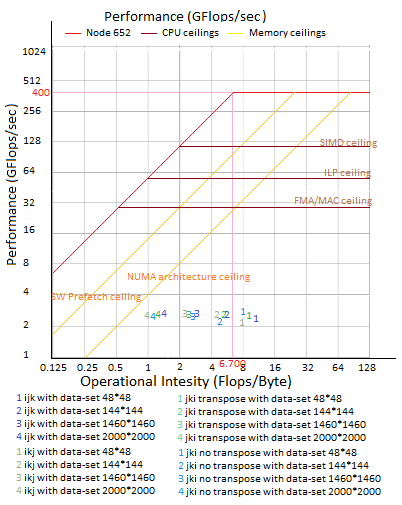
\includegraphics[width=0.50\textwidth, left]{roof3.png}

%The authors would like to thank...


% Can use something like this to put references on a page
% by themselves when using endfloat and the captionsoff option.
\ifCLASSOPTIONcaptionsoff
  \newpage
\fi






% that's all folks
\end{document}








